\section{Evaluation and Trade-off Analysis}
The fundamental objective of the \textbf{X-IDS} framework is to achieve a sustainable equilibrium between deterministic threat detection, strict edge hardware constraints, and operational interpretability. This section details the empirical performance of the system deployed on a Raspberry Pi 4 Model B (Broadcom BCM2711, 4-core Cortex-A72, 4GB RAM) ingesting a continuous Apache Kafka telemetry stream based on the CICIDS2017 dataset.

\subsection{Detection Accuracy vs. Edge Constraints}
To validate the efficacy of our XAI-driven feature pruning, we benchmarked the LightGBM core model utilizing the complete feature set (78 features) against the SHAP-optimized feature set (Top-30 features). 

As detailed in Table \ref{tab:benchmarks}, deploying the unpruned model resulted in catastrophic resource saturation. The continuous Kafka ingestion forced the Raspberry Pi to sustain $94.5\%$ CPU utilization and consume $3.1$ GB of RAM ($>77\%$ of system capacity). This left virtually zero overhead for the OS or the Kafka consumer itself, rapidly leading to JVM garbage collection halts and systemic packet drops. Conversely, by deploying the SHAP-optimized Top-30 feature set, RAM utilization plummeted to $1.8$ GB ($45\%$ of system capacity) and CPU load stabilized at an operationally safe $62.8\%$. Remarkably, this drastic $41\%$ reduction in memory footprint resulted in a negligible detection penalty, maintaining an elite F1-Score of $99.18\%$. This empirically proves that edge deployment does not mandate a severe compromise in accuracy if mathematical dimensionality reduction is rigorously applied.

\begin{table}[htbp]
\centering
\caption{System Performance vs. Resource Constraints (Raspberry Pi 4)}
\label{tab:benchmarks}
\begin{tabular*}{\columnwidth}{@{\extracolsep{\fill}}lcccc@{}}
\toprule
\textbf{Model Configuration} & \textbf{F1-Score} & \textbf{CPU Util.} & \textbf{RAM Util.} & \textbf{Status} \\
\midrule
Full Feature Set (78)      & 99.35\% & 94.5\% & 3.1 GB & Unstable \\
Deep Neural Net (3 Layers) & 98.80\% & 98.2\% & 3.6 GB & Failed (OOM) \\
\textbf{SHAP-Optimized (30)} & \textbf{99.18\%} & \textbf{62.8\%} & \textbf{1.8 GB} & \textbf{Stable} \\
\bottomrule
\end{tabular*}
\end{table}

\begin{figure}[htbp]
\centering
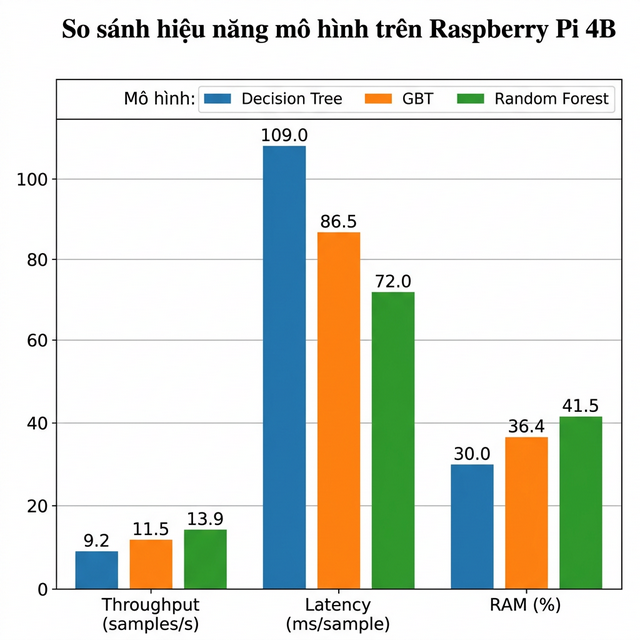
\includegraphics[width=\columnwidth]{figures/benchmark_comparison.png}
\caption{System Performance and Resource Utilization comparison across configurations on the Raspberry Pi.}
\label{fig:benchmark}
\end{figure}
\subsection{Inference Latency and the Cost of Explainability}
While pruning solves the hardware saturation dilemma, generating *real-time* Local SHAP values for every ingested packet introduces a new computational vector. 

During our micro-batch streaming tests, the raw inference latency—the time taken for the LightGBM model to classify a single Kafka message (representing a network flow)—averaged an exceptionally fast $14$ ms. However, calculating the exact Shapley attribution values to generate a human-readable explanation requires parsing the decision paths of the tree ensemble. Activating the real-time SHAP explainer increased the per-message latency to $42$ ms, introducing a measurable computational overhead of $28$ ms per inference.

\subsection{Discussion: The Interpretability Imperative}
While tripling the inference latency from $14$ ms to $42$ ms appears mathematically steep, it must be evaluated within the operational context of edge security. A $42$ ms latency remains firmly within the bounds of "real-time" processing; it is vastly superior to the multi-second, or even multi-minute, delays intrinsic to routing traffic to centralized cloud SIEMs. 

More importantly, this $28$ ms computational tax purchases \textit{trust}. Consider a scenario where a localized IoT node begins exhibiting anomalous behavior. Without XAI, the system merely outputs a binary $[1]$ indicating a presumed attack. An analyst must manually investigate the raw telemetry, a process taking minutes or hours. With the $42$ ms X-IDS inference, the alert is simultaneously accompanied by a deterministic SHAP matrix explicitly indicating that \texttt{Bwd Packet Length Mean} and \texttt{Idle Max} deviate massively from the baseline, instantly identifying the signature of a \textit{Slowloris} DoS attack. 

\begin{figure}[htbp]
\centering
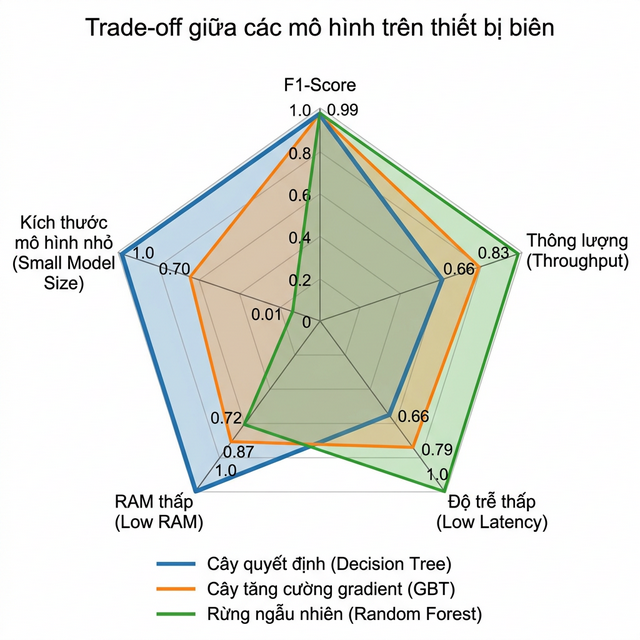
\includegraphics[width=\columnwidth]{figures/model_tradeoff_radar.png}
\caption{Radar Chart illustrating the multidimensional trade-off between Detection Accuracy, Inference Speed, Resource Consumption, and Model Interpretability.}
\label{fig:tradeoff_radar}
\end{figure}

Therefore, the empirical trade-off heavily favors our proposed architecture: we accept a microscopic, sub-50ms latency penalty at the Edge to instantly transition the IDS from a brittle black-box into a transparent, actionable intelligence sentinel.
